
% ----------------------------------------------------------------------
%  Set the document class
% ----------------------------------------------------------------------
\documentclass[11pt,a4paper,twoside]{article}

% ----------------------------------------------------------------------
% Define external packages, language, margins, fonts and new commands
% ----------------------------------------------------------------------
%\input{preamble} 
\usepackage[utf8]{inputenc}   % <<<<< Linux
\usepackage[english]{babel} % <<<<< English
\usepackage{notoccite}
\usepackage[skip=0.05\baselineskip]{caption}
\hyphenation{GTKWave}
\usepackage{listings}
\usepackage[all]{nowidow}
\usepackage{amsmath}
\usepackage{placeins}

%blind text
\usepackage{lipsum}

\usepackage{graphicx}
\graphicspath{ {./} {../../figlib/} }
\def\FontLn{% 16 pt normal
  \usefont{T1}{phv}{m}{n}\fontsize{16pt}{16pt}\selectfont}
\def\FontLb{% 16 pt bold
  \usefont{T1}{phv}{b}{n}\fontsize{16pt}{16pt}\selectfont}
\def\FontMn{% 14 pt normal
  \usefont{T1}{phv}{m}{n}\fontsize{14pt}{14pt}\selectfont}
\def\FontMb{% 14 pt bold
  \usefont{T1}{phv}{b}{n}\fontsize{14pt}{14pt}\selectfont}
\def\FontSn{% 12 pt normal
  \usefont{T1}{phv}{m}{n}\fontsize{12pt}{12pt}\selectfont}

% Use Arial font as default
%
\renewcommand{\rmdefault}{phv}
\renewcommand{\sfdefault}{phv}
\usepackage{geometry}	
\geometry{verbose,tmargin=2.5cm,bmargin=2.5cm,lmargin=2.5cm,rmargin=2.5cm}
\usepackage{mathtools}
%\usepackage{setspace}
%\renewcommand{\baselinestretch}{1.5}

\usepackage[pdftex]{hyperref} % enhance documents that are to be
                              % output as HTML and PDF
\hypersetup{colorlinks,       % color text of links and anchors,
                              % eliminates borders around links
%            linkcolor=red,    % color for normal internal links
            linkcolor=black,  % color for normal internal links
            anchorcolor=black,% color for anchor text
%            citecolor=green,  % color for bibliographical citations
            citecolor=black,  % color for bibliographical citations
%            filecolor=magenta,% color for URLs which open local files
            filecolor=black,  % color for URLs which open local files
%            menucolor=red,    % color for Acrobat menu items
            menucolor=black,  % color for Acrobat menu items
%            pagecolor=red,    % color for links to other pages
            pagecolor=black,  % color for links to other pages
%            urlcolor=cyan,    % color for linked URLs
            urlcolor=black,   % color for linked URLs
	          bookmarks=true,         % create PDF bookmarks
	          bookmarksopen=false,    % don't expand bookmarks
	          bookmarksnumbered=true, % number bookmarks
	          pdftitle={report},
            pdfauthor={Andre C. Marta},
%            pdfsubject={Thesis Title},
%            pdfkeywords={Thesis Keywords},
            pdfstartview=FitV,
            pdfdisplaydoctitle=true}

\usepackage[numbers,sort&compress]{natbib} % <<<<< References in numbered list [1],[2],...
\usepackage{subcaption} 
\usepackage{mdframed}
\usepackage{float}
%%%%%%%%%%%%%%%%%%%%%%%%%%%%%%%%%%%%%%%%%%%%%%%%%%%%%%%%%%%%%%%%%%%%%%%%
%     Begin Document                                                   %
%%%%%%%%%%%%%%%%%%%%%%%%%%%%%%%%%%%%%%%%%%%%%%%%%%%%%%%%%%%%%%%%%%%%%%%%


\begin{document}

% Set plain page style (no headers, footer with centered page number)
\pagestyle{plain}

% Set roman numbering (i,ii,...) before the start of chapters
%\pagenumbering{roman}

% ----------------------------------------------------------------------
%  Cover page
% ----------------------------------------------------------------------
%%%%%%%%%%%%%%%%%%%%%%%%%%%%%%%%%%%%%%%%%%%%%%%%%%%%%%%%%%%%%%%%%%%%%%%%
%                                                                      %
%     File: Thesis_FrontCover.tex                                      %
%     Tex Master: Thesis.tex                                           %
%                                                                      %
%     Author: Andre C. Marta                                           %
%     Last modified :  2 Jul 2015                                      %
%                                                                      %
%%%%%%%%%%%%%%%%%%%%%%%%%%%%%%%%%%%%%%%%%%%%%%%%%%%%%%%%%%%%%%%%%%%%%%%%

\thispagestyle {empty}

% IST Logo - Signature A
% parameters: bb=llx lly urx ury (bounding box), width=h_length, height=v_length, angle=angle, scale=factor, clip=true/false, draft=true/false. 
\includegraphics[bb=9.5cm 11cm 0cm 0cm,scale=0.29]{IST_A_CMYK_POS.pdf}

\begin{center}
%
% Figure (Image or plot)
\vspace{1.0cm}
% height = 50 mm
%\includegraphics[height=50mm]{Figures/Airbus_A350.jpg}

% Title, author and degree
\vspace{1cm}
{\FontLb Circuit Theory and Electronics Fundamentals} \\ % <<<<< EDIT TITLE
\vspace{3cm}
{\FontSn T2 Laboratory Report} % <<<<< EDIT COURSE
\vspace{3cm}
\par
{\FontSn Aerospace Engineering, Técnico, University of Lisbon} \\
\vspace{1cm}
{\FontSn April 8, 2021}\\ % <<<<< EDIT DATE (corresponds to date of oral examination)
%
\vspace{1.5cm}
{\FontLb Group 19} \\
\vspace{1cm}
{\FontSn João Silva, n° 95802} \\
{\FontSn Miguel Cunha, n° 95832} \\
{\FontSn Frederico Baptista, n° 97196} \\
\end{center}

\pagebreak
% ----------------------------------------------------------------------
% Dedication page (optional)
% ----------------------------------------------------------------------
%\input{dedication} 
%\cleardoublepage

% ----------------------------------------------------------------------
%  Acknowledgments (optional)
% ----------------------------------------------------------------------
%\input{acknowledgements}
%\cleardoublepage

% ----------------------------------------------------------------------
%  Abstract (both in English and Portuguese)
% ----------------------------------------------------------------------
%\input{resumo} 
%\cleardoublepage

%\input{abstract} 

% ----------------------------------------------------------------------
%  Table of contents, list of tables, list of figures and nomenclature
% ----------------------------------------------------------------------
% Table of contents
%
\tableofcontents
\vspace{1cm}
\pagebreak


\section{Introduction}
\label{sec:introduction}

% state the learning objective 
The objective of this laboratory assignment is to choose the dimensions and implement a BandPass Filter (BPF) with the a central frequency of 1kHz and a gain of 40dB (at central frequency). \par
\vspace{0.5cm}
The components used:\par
– One 741 OPAMP; \par
– At most three 1k$\Omega$ resistors; \par
– At most three 10k$\Omega$  resistors; \par
– At most three 100k$\Omega$  resistors; \par
– At most three 220nF capacitors;\par
– At most three 1$\mu$ F capacitors; \par
\vspace{0.5cm}
The bandpass filter was simulated using Ngspice, based on the script given, using the provided OPAMP model. This simulation is design to measure the output voltage gain in the passband, the central frequency and the input and output impedances at this frequency. \par
The merit was then worked on with some modifications. \par
The merit is calculated using: \par
\begin{equation}
    M = \frac{1}{Cost \times (gain_{deviation} + CentralFrequency_{deviation} + 10^{-6})}
\end{equation}\par
Where:\par
- cost = cost of resistors + cost of capacitors + cost of transistors; \par
– cost of resistors = 1 monetary unit (MU) per kOhm; \par
– cost of capacitors = 1 MU/$\mu$ F; \par
– cost of transistors = 0.1 MU per transistor; \par
\vspace{0.5cm}
Using octave, both the gain, input and the output impedances were computed at the central frequency, since we were analysing a BandPass Filter. \par
Frequency response $V_{o}(f)/V_i{f}$ was also computed, using the incremental analysis, solving the circuit for a frequency vector in log scale with 10 points per decade, from 10Hz to 100MHz.\par
\par In this assignment, the merit obtained is around $3.3 \cdot 10^{-6}$, the central frequency is 718Hz, with a gain of 34dB. Not the best values, but close to the objective, while allowing for a great learning experience.\par

It was used an incremental method in order to improve the figure of merit. Starting with a simple circuit and continuously updating it. The final circuit is shown bellow (Fig.\ref{fig:circuito}): \par

\begin{figure}[H]
\centering
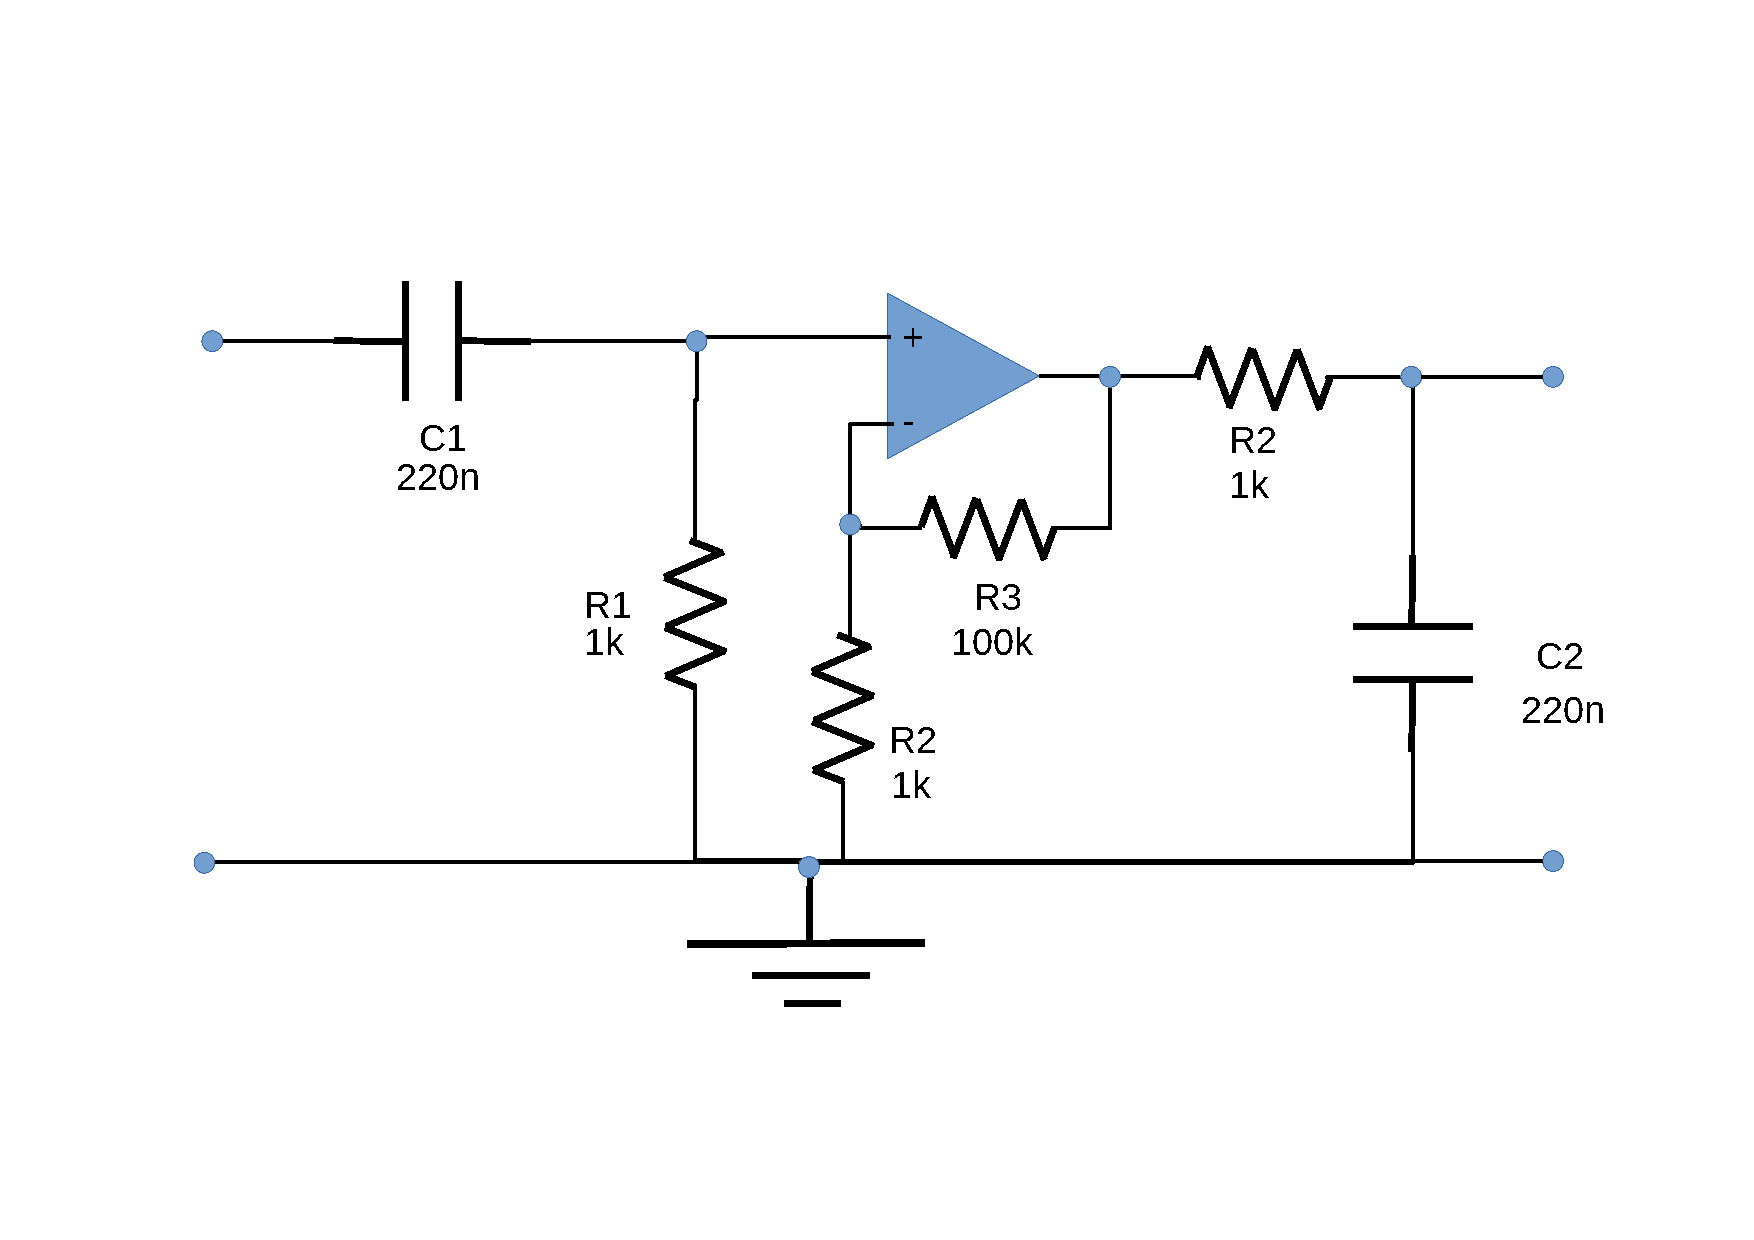
\includegraphics[width=0.9\linewidth]{circuito}
\caption{Final circuit}
\label{fig:circuito}
\end{figure}

The individual costs of the components used: 

\begin{center}
  \begin{tabular}{ | c | c | }
    \hline    
    {\bf Name} & {\bf Value} \\ \hline
    $R$ & 103k$\Omega$ \\ \hline 
    $C$ & 0.440 $\mu$C \\ 
    \hline
  \end{tabular}
  \captionof{figure}{Costs}
\end{center}

\newpage

\section{Theoretical Analysis}

In this section, the circuit shown in Figure \ref{fig:Circuit} is analysed
theoretically using both the Mesh Method and Nodal Method.

\label{sec:analysis}
\subsection {{Mesh Method}}
For the Mesh Method, circular currents are introduced in the different single meshes of the circuit as shown in \ref{fig:MeshAnalysis} and then the circuit is evaluated considering those new currents.

\begin{figure}[h] \centering
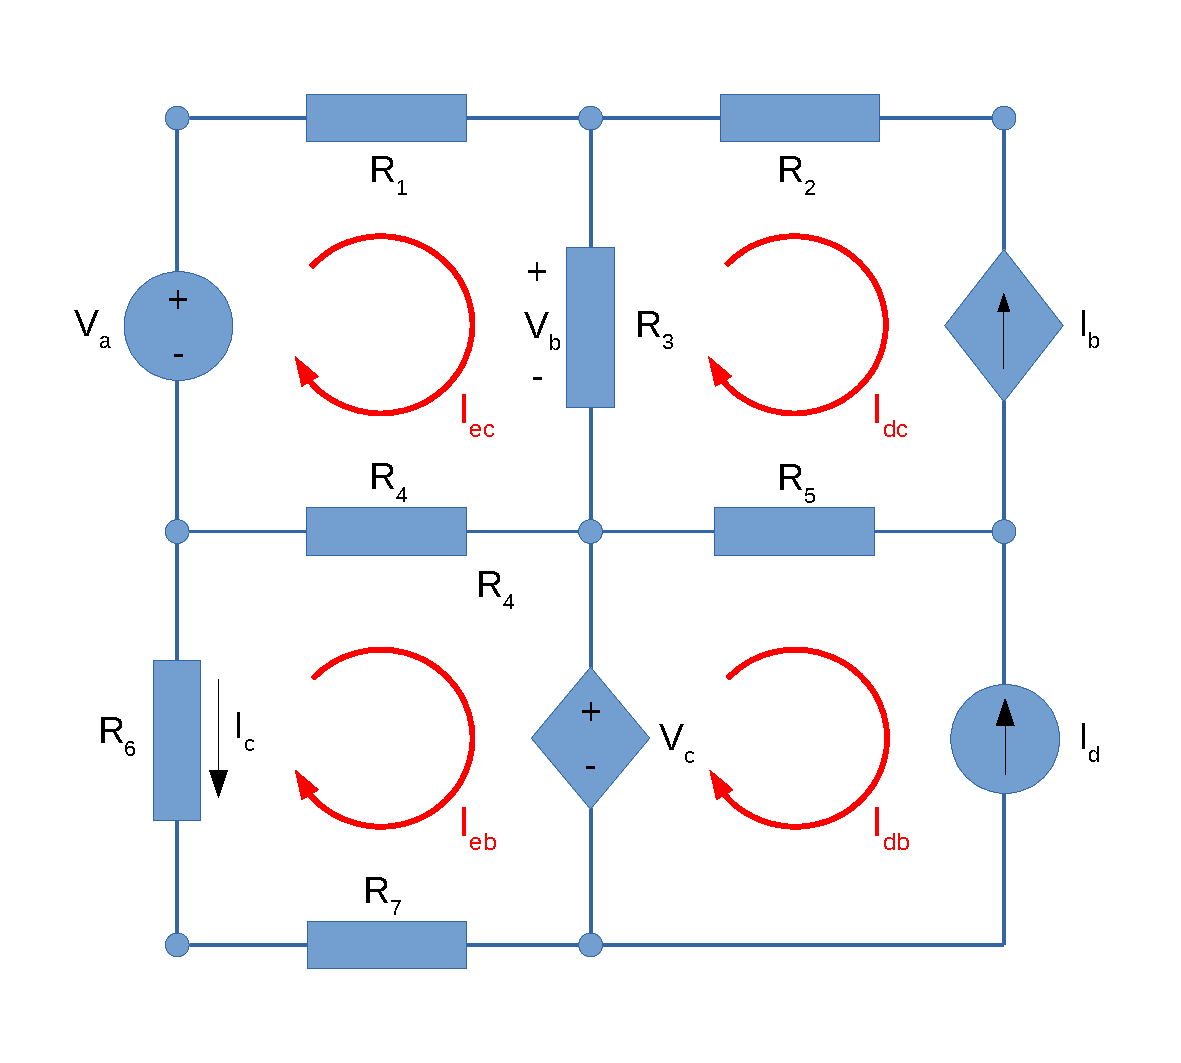
\includegraphics[width=0.4\linewidth]{MeshAnalysis.pdf}
\caption{Mesh Analysis}
\label{fig:MeshAnalysis}
\end{figure}

After identifying all the mesh currents, considering the above, it is now necessary to use Kirchhoff Voltage Law (KVL) in those meshes that don't contain current sources (Mesh EC (\textbf{\ref{eq:KVL_{ec}}}) and EB (\textbf{\ref{eq:KVL_{eb}}})) and relate the mesh currents to those imposed by the sources (Mesh DC (\textbf{\ref{eq:KVL_{dc}}}) and DB (\textbf{\ref{eq:KVL_{db}}}).

\vspace{0.1cm}

\begin{equation}
 -V_{a} + R_{1} I_{ec} + V_{b} + R_{4} (I_{ec} - I_{eb}) = 0
 \label{eq:KVL_{ec}}
\end{equation}

\begin{equation}
    I_{dc} = -I_{b}
    \label{eq:KVL_{dc}}
\end{equation}

\begin{equation}
     I_{db} = -I_{d}
     \label{eq:KVL_{db}}
\end{equation}

\begin{equation}
     V_{c} + R_{7} I_{eb} + R_{6} I_{eb} + R_{4} (I_{eb} - I_{ec}) = 0
      \label{eq:KVL_{eb}}
\end{equation}

\vspace{0.1cm}
Analysing the equations it is noticeable that we have 8 variables and that we'll need four more equations to solve the circuit. It is, also, important to notice that two of them are already given:
\begin{equation}
    V_{c} = K_{c} I_{c}
\end{equation}

\begin{equation}
    I_{b} = K_{b} V_{b}
\end{equation}

\vspace{0.1cm}
The other two are trivial equations found by the careful examination of the circuit with Ohm's Law:
\vspace{0.1cm}
\begin{equation}
    I_{c} = -I_{eb}
\end{equation}

\begin{equation}
    V_{b} = R_{3} (I_{ec} - I_{dc})
\end{equation}

\pagebreak
In the following table, both current and voltage for each component are presented:
\begin{center}
\begin{tabular}{ |c|c|c| }
 \hline
\textbf{Name} & \textbf{Current (A)} & \textbf{Tension (V)} \\
 \hline
 $I_{EC}$ & 2.143086e-04 & - \\ \hline 
$I_{DC}$ & 2.241280e-04  & -\\ \hline 
$I_{DB}$ & -1.024396e-03  & -\\ \hline 
$I_{EB}$ & -9.691453e-04  & -\\ \hline 
$V_{b}$ & - & -3.068815e-02 \\ \hline 
$V_{c}$ & - & 7.881834e+00 \\ \hline 
$I_{b}$ & -2.241280e-04  & -\\ \hline 
$I_{c}$ & 9.691453e-04  & -\\ \hline 

\end{tabular}
\end{center}

\subsection{Nodal Metod}
To determine the values of the current and voltage using the Nodal Method it is first necessary 
to find all the knots in the circuit, as shown in \ref{fig:NodeAnalysis}.

\begin{figure}[h] \centering
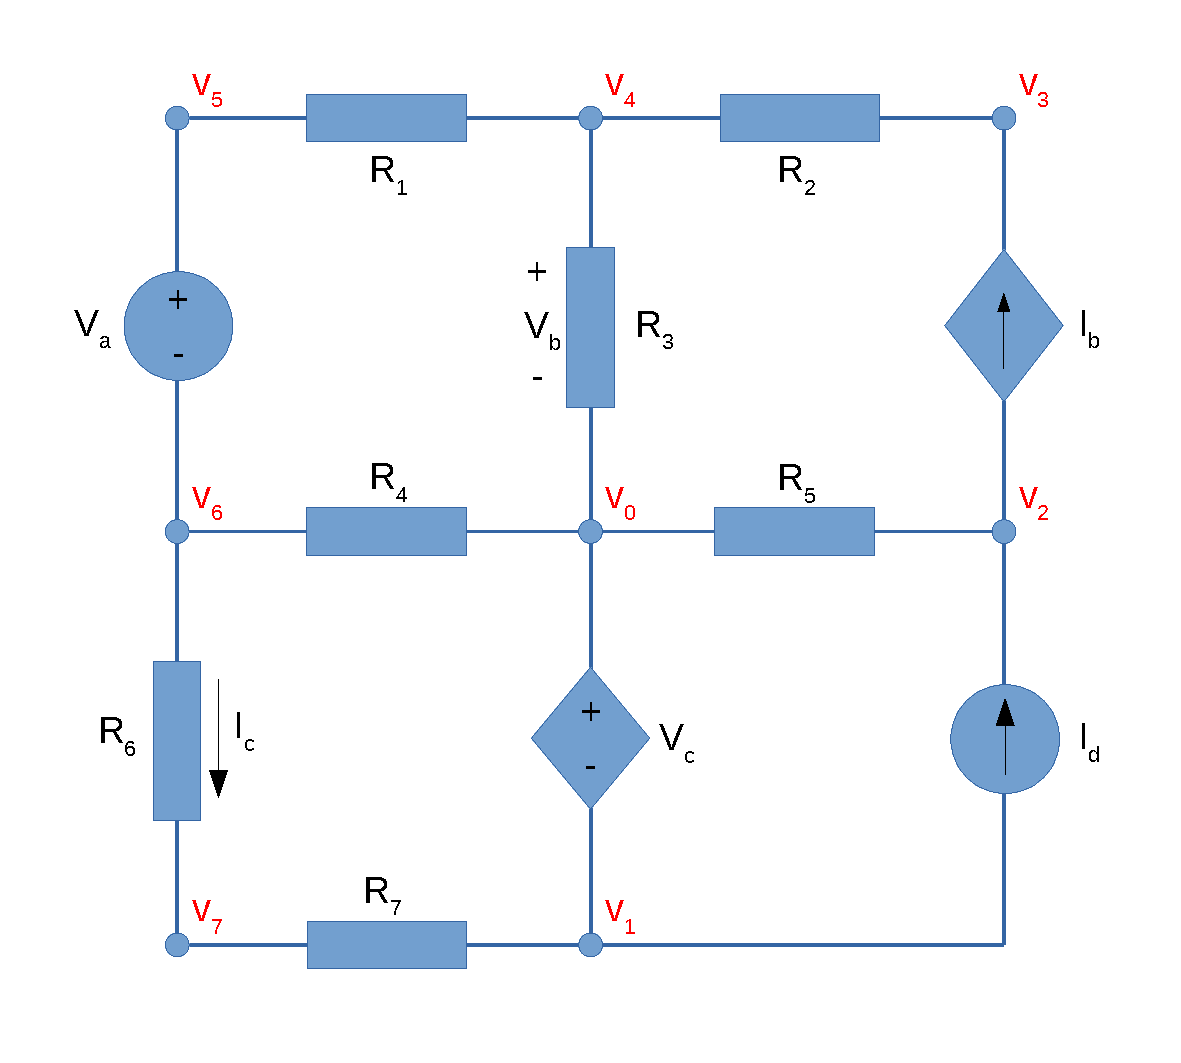
\includegraphics[width=0.4\linewidth]{NodeAnalysis.pdf}
\caption{Node Analysis}
\label{fig:NodeAnalysis}
\end{figure}


The Kirchhoff Current Law (KCL) is then used in the nodes that are not connected
to voltage sources (from \ref{eq:KCL_{9}} to \ref{eq:KCL_{12}})
\vspace{0.1cm}
\begin{equation}
    V_{5} G_{1} - V_{4} (G_{1} + G_{2}) + V_{3} G_{2} - V_{b} G_{3} = 0
    \label{eq:KCL_{9}}
\end{equation}

\begin{equation}
    -V_{3} G_{2} + V_{4} G_{2} + I_{b} = 0
\end{equation}

\begin{equation}
    V_{2} G_{5} + V_{0} G_{5} + I_{d} = I_{b}
\end{equation}

\begin{equation}
    G_{6} (V_{6} - V_{7}) - I_{c} = 0
    \label{eq:KCL_{12}}
\end{equation}
\vspace{0.5cm}

\pagebreak

In \ref{eq:KCL_{13}} and \ref{eq:KCL_{14}}, a relationship is established between
a knot's voltage and the voltage sources that are connected to them:

\begin{equation}
    V_{5} - V_{6} = V_{a}
    \label{eq:KCL_{13}}
\end{equation}

\begin{equation}
    V_{c} = V_{0} - V_{1}
    \label{eq:KCL_{14}}
\end{equation}



\vspace{0.5cm}

By analysing the circuit we get:

\vspace{0.5cm}
\begin{equation}
    V_{c} = K_{c} I_{c}
\end{equation}

\begin{equation}
    I_{b} = K_{b} V_{b}
\end{equation}

\begin{equation}
    V_{b} = V_{4} - V_{0}
\end{equation}

\begin{equation}
    V_{0} = 0
\end{equation}


Using Ohm's Law:

\begin{equation}
    I_{c} = V_{6} G_{6} - V_{7} G_{6}
\end{equation}
\vspace{0.5cm}


The continuity of current in voltage sources allows to write this equation:
\begin{equation} 
    V_{5} G_{1} - V_{4} G_{1} + I_{c} + V_{0} G_{4} - V_{6} G_{4} = 0   
\end{equation}

In the following table, both current and voltage for each component are presented:
\begin{center}
\begin{tabular}{ |c|c|c| }
 \hline
\textbf{Name} & \textbf{Current (A)} & \textbf{Tension (V)} \\
 \hline
 $v_{0}$ & 0.000000e+00 \\ \hline 
$v_{1}$ & -7.881834e+00 \\ \hline 
$v_{2}$ & 3.805553e+00 \\ \hline 
$v_{3}$ & -4.970348e-01 \\ \hline 
$v_{4}$ & -3.068815e-02 \\ \hline 
$v_{5}$ & 1.871742e-01 \\ \hline 
$v_{6}$ & -4.894946e+00 \\ \hline 
$v_{7}$ & -6.897288e+00 \\ \hline 
$V_{b}$ & -3.068815e-02 \\ \hline 
$V_{c}$ & 7.881834e+00 \\ \hline 
$I_{b}$ & -2.241280e-04 \\ \hline 
$I_{c}$ & 9.691453e-04 \\ \hline 

\end{tabular}
\end{center}

\pagebreak







\section{Simulation Analysis}
\label{section:sim}
 
In this section, the several steps taken using ngspice in order to conduct the simulation of the audio amplifier, as requested, will be described. The main focus of the simulation was to determine and optimize the values of the gain, the cut off frequencies, both lower and upper and the bandwidth. The quality and overall figure of merit will then be analysed.
The group proceded as follows:

\begin{enumerate}
\item Design of the circuit, having as a starting point the circuit given by the professor.

\item Verification of the operation of the transistors in the forward Active region, the called F.A.R mode. The results are shown below.

\begin{table}[ht]
  \centering
  \begin{tabular}{|l|r|}
    \hline    
   \input{../sim/NPN_tab} %../sim/NPN_tab
     \end{tabular}
  \caption{Verification of the F.A.R mode in the NPN transistor}
 
\end{table}


\begin{table}[ht]
  \centering
  \begin{tabular}{|l|r|}
    \hline    
   \input{../sim/PNP_tab} %../sim/PNP_tab
     \end{tabular}
  \caption{Verification of the F.A.R mode in the NPN transistor}
    
\end{table}



\item OP Analysis
\par Then, the OP values of the currents and nodal voltages were computed. These are key to calculate the incremental parameters.

  
\item  In the frequency domain, measure of the output voltage gain, using the function .meas as well as the lower and upper cut off frequencies and the bandwidth.


\begin{table}[ht]
  \centering
  \begin{tabular}{|l|r|}
    \hline    
   \input{../sim/results_tab} %../sim/
    \end{tabular}
  \caption{Results for ngspice}
    \label{tab:results}
\end{table}


The quantities obtained are desribed in the table \ref{tab:results}. The results obtained allowed the group to understand the functions of the different components of the circuit. 
The conclusions will be outlined.


 \textbf{EFFECT OF THE COUPLING CAPACITORS}

The coupling capacitors' main porpuse is to block the DC signals. If studying an incremental model of an audio amplifier, all values that are constant must be eliminated so the transistors are always fowardly conducting. As so, two coupling capacitors were used. Once the capacitors may also block some low frequencies, they have a direct influence in the bandwidth.



 \textbf{EFFECT OF THE BYPASS CAPACITOR}
 
  As studied in the lectures, the resistor Re has the funciton of stabelizing the effect of the temperature in the DC voltage. However, it has also a negative effect on the gain, once it lowers it. In order to solve the problem, a bypass capacitor Ce is placed in parallel with the resistor, so that the capacitor bypasses the resistor. In DC mode, the resistor plays its effect in the temperature. In AC, the resistor will not affect the gain. To sum up, the capacitor is a short-circuit for higher frequencies (AC) and a open-circuit for low frequencies (DC).



 \textbf{EFFECT OF RC}
 
IC is the most important current in the circuit because it determines gm, and so directly influences the gain, by increasing it.

\textbf{GRAPHICAL REPRESENTATION}

In the graphics \ref{fig:sim4} and \ref{fig:sim5}, a graphic representation of the effect of the components above mentioned can be observed. In fact, in the plot \ref{fig:sim5} is extremely enlightening as one can intuitevely notice the high bandwidth, the stabilization of the gain, and the gain itself.




\begin{figure}[ht]
\centering
\begin{subfigure}{.5\textwidth}
  \centering
  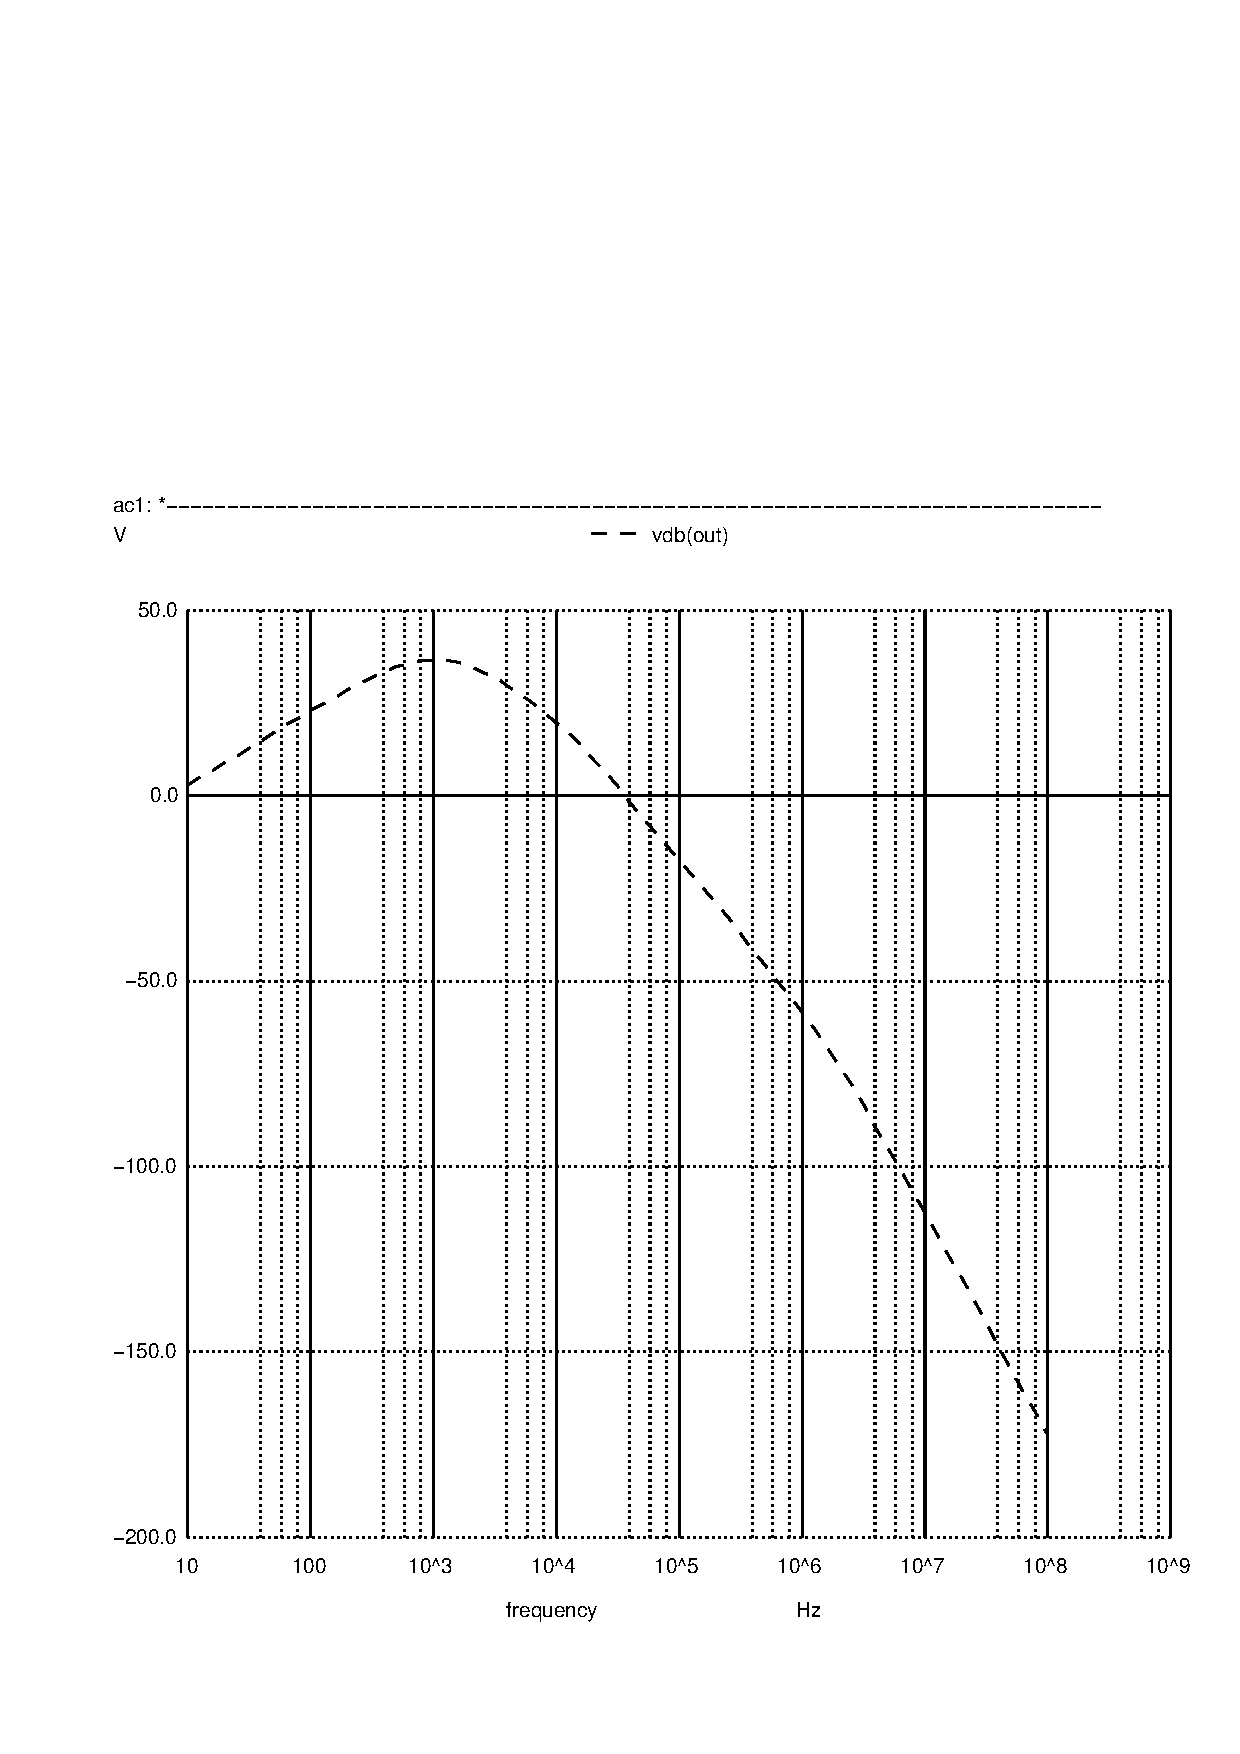
\includegraphics[width=.75\linewidth]{../sim/vo1f.pdf}
  \caption{Input Voltage}
  \label{fig:sim4}
\end{subfigure}%
\begin{subfigure}{.5\textwidth}
  \centering
  \includegraphics[width=.75\linewidth]{../sim/vo2f.pdf}
  \caption{Output voltage}
  \label{fig:sim5}
\end{subfigure}
\end{figure}




\item Determination of the input impedance, seen from the input voltage source.

\begin{table}[h]
  \centering
  \begin{tabular}{|l|r|}
    \hline    
   \input{../sim/Zin_tab} %../sim/
   \end{tabular}
  \caption{Input impedance in Ohm}
    \label{tab:ZI}
\end{table}

\par The result obtained for the input impedance, considering the value in Ohm, is high. This is benefitial for the gain, because the voltage in the node In 2 must be as similiar to Vin as possible. Using a voltage divider, the only way to achieve this was to have a very high resistance value.

\item Determination of the output impedance, using a different set up, seen from the load resistance. 

\begin{table}[h]
  \centering
  \begin{tabular}{|l|r|}
    \hline    
   \input{../sim/op_ZO_tab} %../sim/
   \end{tabular}
  \caption{Output impedance in Ohm}
  
  \label{tab:ZO}
\end{table}


Conserning the output impedance, an opposite deduction to the one made for the output impedance is mandoratory. Considering a voltage divider, the output impedance must be as low as possible, in order to the output voltage to be as high as possible. Having said that, an analysing tables \ref{tab:ZI} and \ref{tab:ZO}, the difference needed between the two is confirmed. The output impedance obtained is reasonable compared to the 8 Ohm load resistance. (About 8 times higher)

\item Compute of the cost and figure of merit
\par To finally understand the efficency of the amplifier, the cost and figure of merit were calculated

\begin{table}[ht]
  \centering
  \begin{tabular}{|l|r|}
    \hline    
   \input{../sim/cost_tab} %../sim/
   \end{tabular}
  \caption{Cost and Figure of merit}
  \label{tab:cost}
\end{table}

Analysing table \ref{tab:cost}, the results obtained may be considered satisfying.


\end{enumerate}




\section{Conclusion}
\label{sec:conclusion}

This assignment made us understand how a band pass filter work and how an OP-AMP circuit relates to and the band and the voltage gain.\par
As it can be noticed, there are some differences between the theoretical and simulation values obtained, this is the case for the OP analysis and also the impedances. This difference is explained by the use of non-linear components (transistors) that make the OP analysis deviate from the theoretical analysis. Since the linear components have constant circuit parameters, it is really easy for Ngspice to plot and analyse them in perfection in relationship to the theorethical calculations. It cannot be said the same thing for non-linear components, once those circuit parameters vary. \par
The merit figure as explained before was a very important part of this assignment, since it provides a relation with the "real world" where everything as a cost and a energy consumption, so it was important that this value was the most accurate as possible. In order to achieve that, the Ngspice's result was used. \par
As it can be way easier to compare, it is shown below the results from simulation and theoretical analysis side by side: \par
%compararações

\section{Visual Data}
\label{sec:data}

\begin{center}
  \begin{tabular}{ | c | c | }
    \hline    
    {\bf Name} & {\bf Value} \\ \hline
    merit & 1.580376e-03\\ \hline

  \end{tabular}
  \captionof{figure}{Merit Figure Table}
\end{center}

\begin{center}
  \begin{tabular}{ | c | c | }
    \hline    
    {\bf Name} & {\bf Value [$Hz$ or $dB$]} \\ \hline
    central & 9.973752e+02\\ \hline
voltagegain & 3.650113e+01\\ \hline

    \hline
  \end{tabular}
  \captionof{figure}{Central Frequency, Voltage Gain - Simulation}
\end{center}

\begin{center}
  \begin{tabular}{ | c | c | }
    \hline    
    {\bf Name} & {\bf Value [$Hz$ or $dB$]} \\ \hline
    Central Frequency & 8.141678e+02 \\ \hline 
Voltage Gain dB & 3.964755e+01 \\ 

    \hline
  \end{tabular}
  \captionof{figure}{Central Frequency, Voltage Gain - Theoretical}
\end{center}

\begin{figure}[H]
    \minipage{0.45\textwidth}
      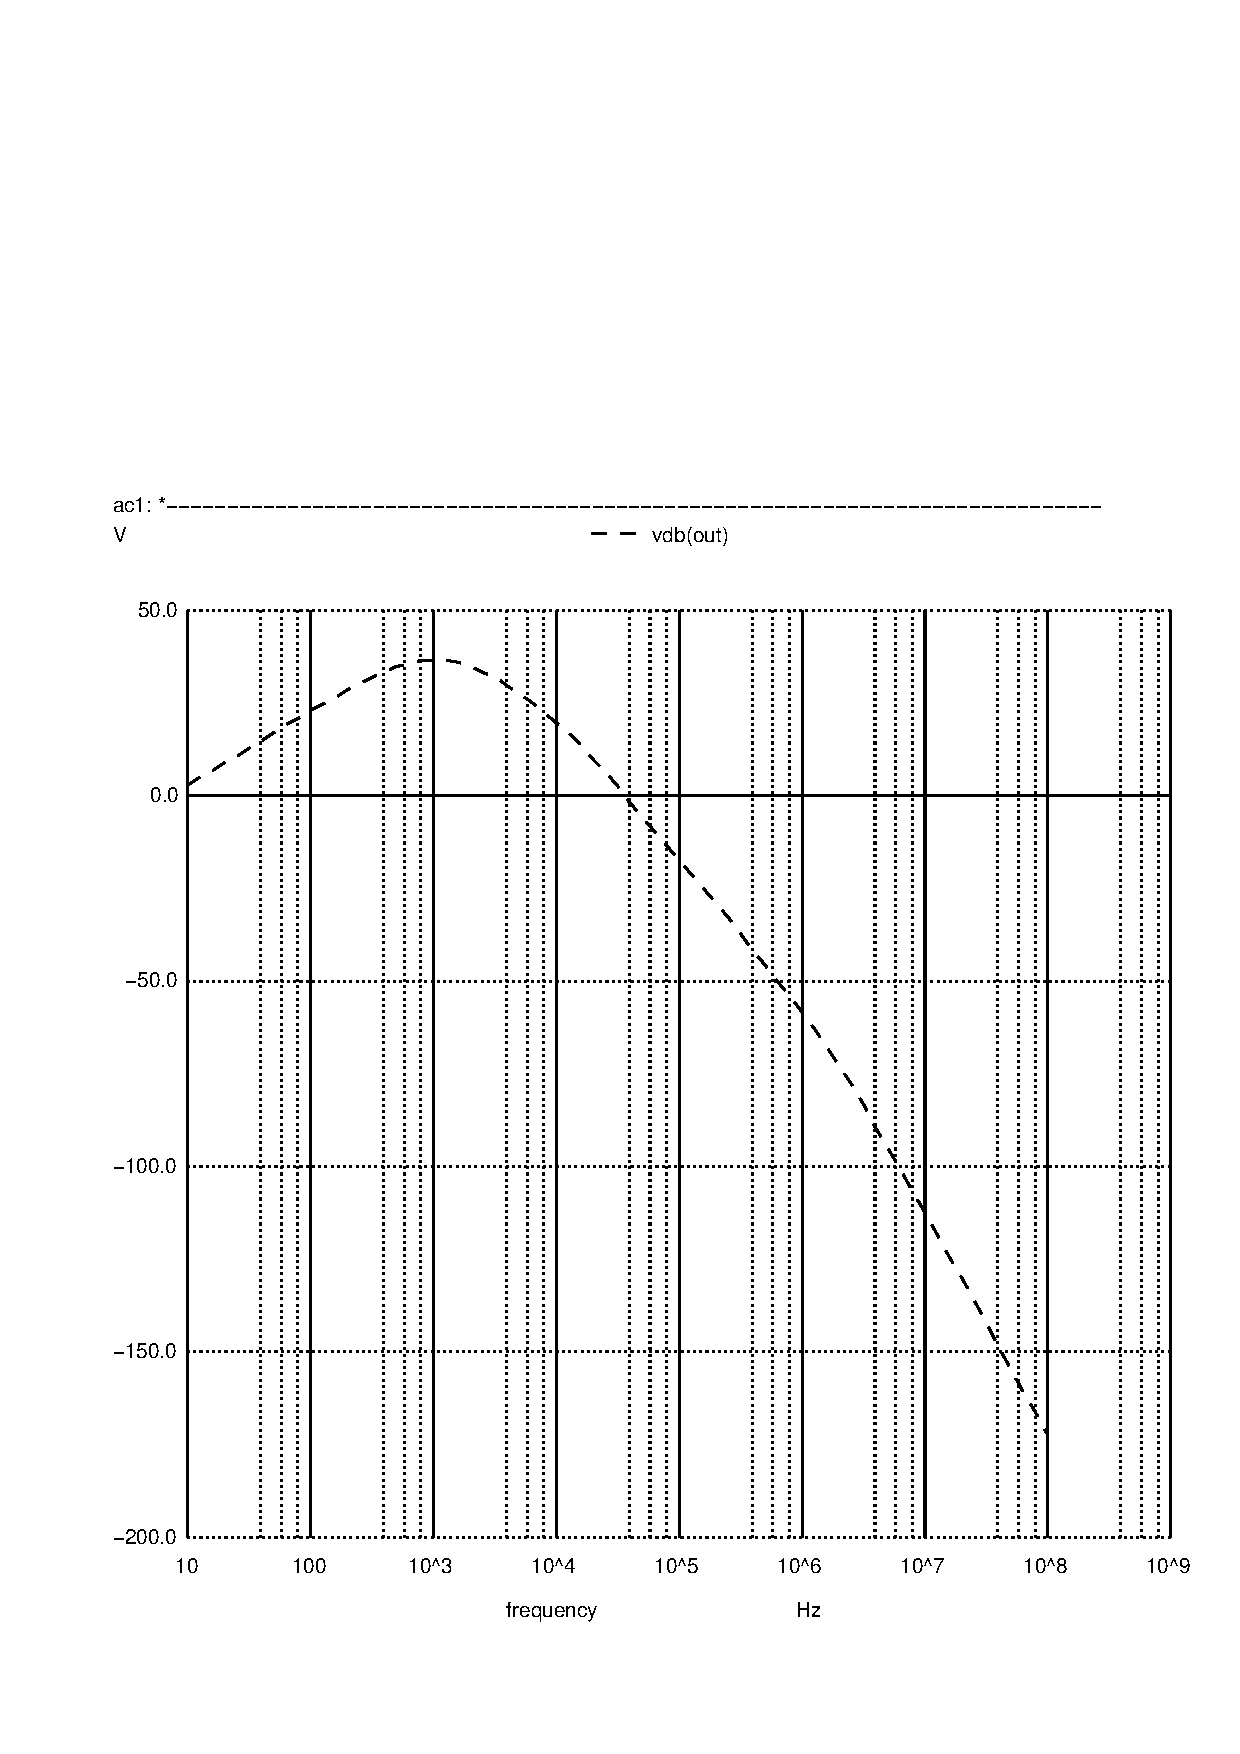
\includegraphics[width=\linewidth]{../sim/vo1f.pdf}
      \caption{Simulation Gain Frequency Response - $dB$}
    \endminipage\hfill
    \minipage{0.45\textwidth}
      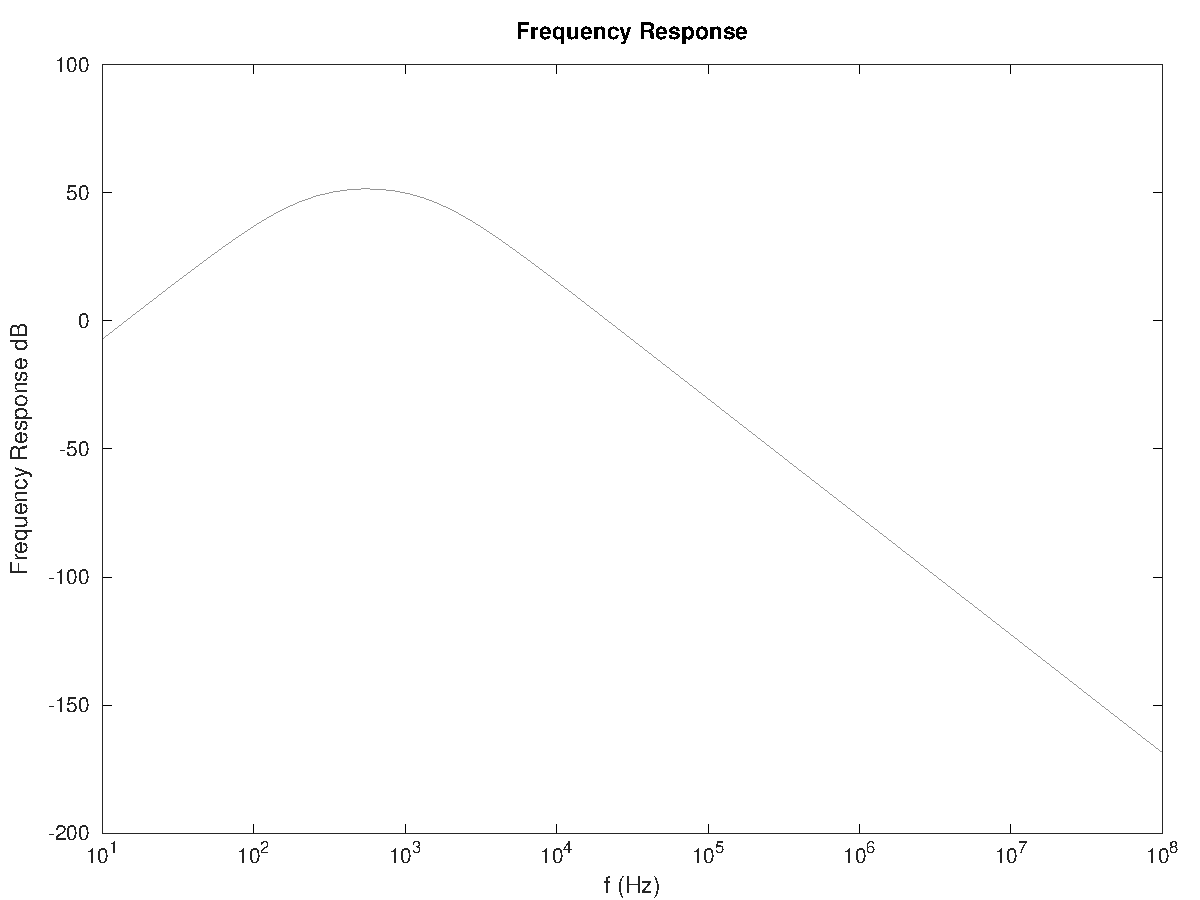
\includegraphics[width=\linewidth]{../mat/fresponse1.pdf}
      \caption{Theoretical Gain Frequency Response - $dB$}
    \endminipage\hfill
\end{figure}


\begin{figure}[H]
    \minipage{0.45\textwidth}
      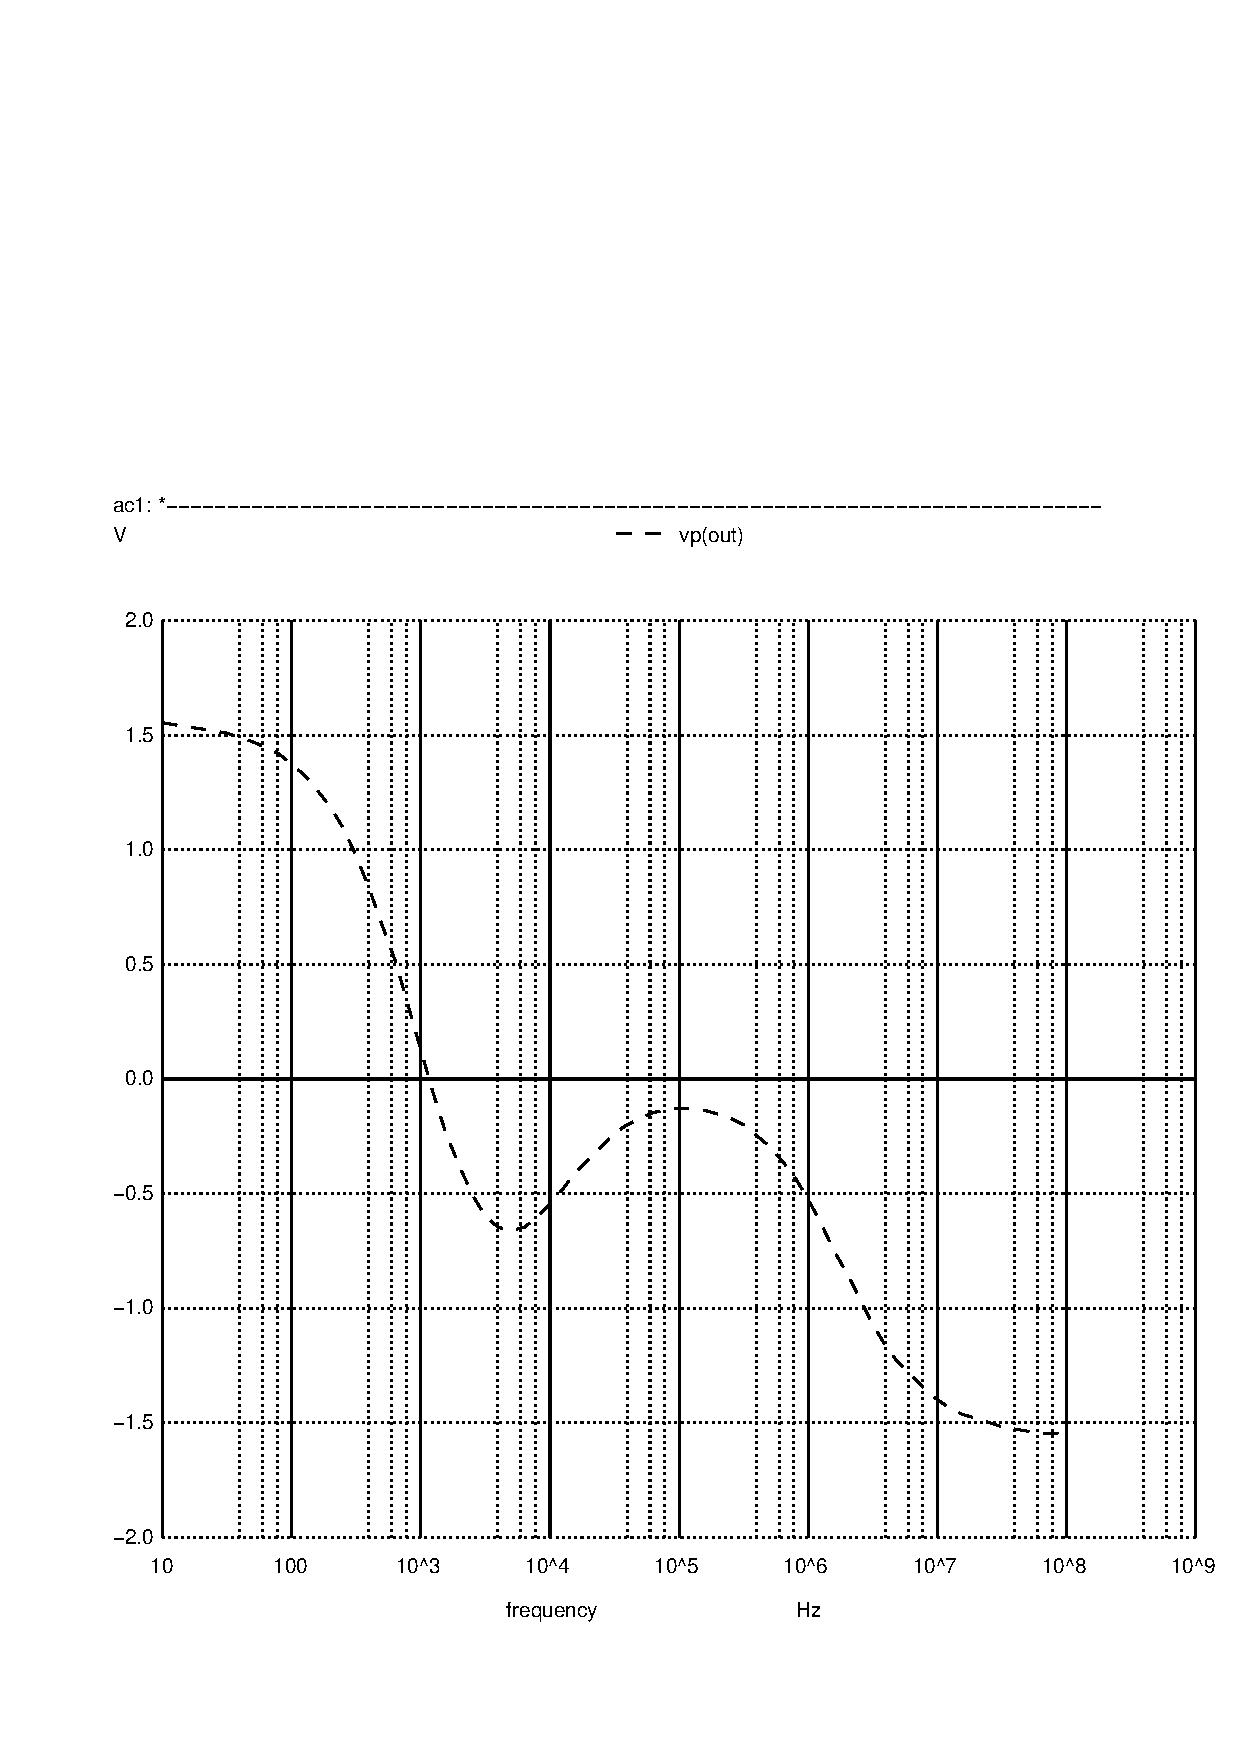
\includegraphics[width=\linewidth]{../sim/vo1p.pdf}
      \caption{Simulation Gain Frequency Response - Phase}
    \endminipage\hfill
    \minipage{0.45\textwidth}
      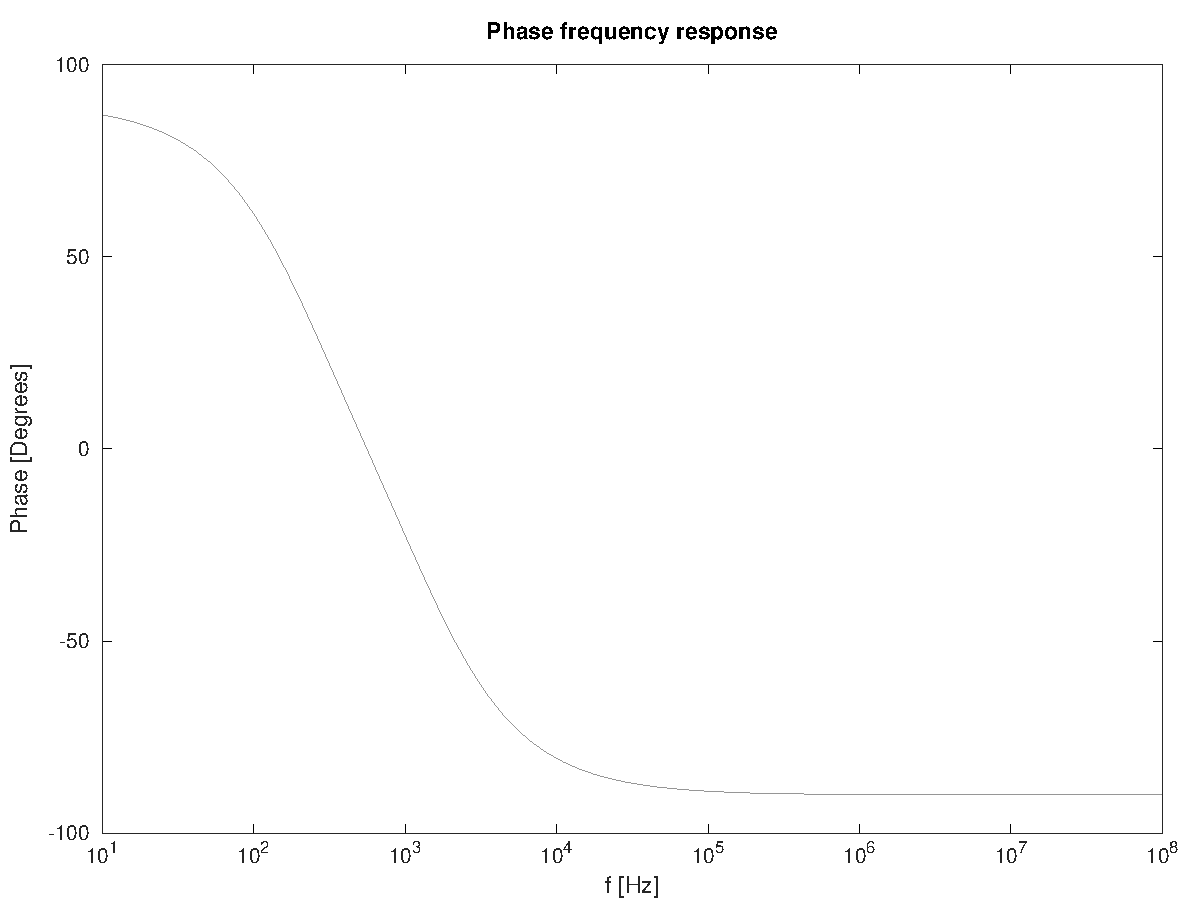
\includegraphics[width=\linewidth]{../mat/fresponse2.pdf}
      \caption{Theoretical Gain Frequency Response - Phase}
    \endminipage\hfill
\end{figure}


\begin{center}
  \begin{tabular}{ | c | c | }
    \hline    
    {\bf Name} & {\bf Value [$\Omega$]} \\ \hline
    inputimpedance & -9.99987e+02,7.233281e+02\\ \hline

  \end{tabular}
  \captionof{figure}{Simulation Input Impedance}
\end{center}

\begin{center}
  \begin{tabular}{ | c | c | }
    \hline    
    {\bf Name} & {\bf Value [$\Omega$]} \\ \hline
    Output Impedance & 345.125 + -475.63 j\\ \hline

  \end{tabular}
  \captionof{figure}{Simulation Output Impedance}
\end{center}

\begin{center}
  \begin{tabular}{ | c | c | }
    \hline    
    {\bf Name} & {\bf Value [$\Omega$]} \\ \hline
    Input Impedance & 5.000000e+02 \\ \hline 
Output Impedance & 2.396034e+02 \\ 

    \hline
  \end{tabular}
  \captionof{figure}{Theoretical Input and Output Impedances}
\end{center}
%\cleardoublepage

% ----------------------------------------------------------------------
%  Bibliography
% ----------------------------------------------------------------------
%\addcontentsline{toc}{section}{\bibname}
%\bibliographystyle{abbrvunsrtnat} % <<<<< SELECT IF USING REFERENCES BY NUMBER (CITATION ORDER)
%\bibliography{../../../BIBfile.bib}

% ----------------------------------------------------------------------
\end{document}
% ----------------------------------------------------------------------
